\section*{Supplementary Information}
\label{sec:si}

This supplement gives the implementation details and sensitivity results that
are needed to reproduce the study but are not needed to follow the main paper.
It covers the image and semantic-model roles, street-image acceptance, numerical settings,
provenance, convergence, the material-evidence control, timing boundaries, and
additional limitations. Unless marked as the separate fixed-grid diagnostic,
numerical statements refer to the verified five-site calculations under the
first-material-interaction transport contract.

\section{Image labels and material mapping}
\label{sec:si-semantics}

The image-labeling pass uses two models with separate roles. Mask2Former with the
65-class Mapillary Vistas vocabulary assigns one street-scene object class to every pixel. It
therefore supplies the complete object map and identifies small objects such
as poles, signs, curbs, and bicycle racks. One Vistas building label can contain
brick, stone, render, glass, and metal. SAM~3 supplies the open-vocabulary
material labels needed inside such broad object classes. The production
catalog contains 60 text prompts and 61 raster identifiers including the
unlabeled identifier. Examples include ``brick facade'', ``glass window'',
``metal cladding panel'', and separate ground, grass, shrub,
tree, and forest concepts. The prompts are also gated by the Vistas classes. A class
must occupy at least 256 pixels in a $1536\times1536$ crop before its related
prompts are sent to SAM~3. The gate reduces work and removes prompts that have no
matching object in the view. The complete prompt list and its object, material,
attribute, and vegetation mappings are stored in
\texttt{config/semantic\_concepts.json}.

The four rectilinear crops of each 360-degree street image face $0^\circ$,
$90^\circ$, $180^\circ$, and $270^\circ$, zero pitch, a $90^\circ$ field of
view, and $1536$ pixels per side. Mask2Former runs at $1536$ pixels. SAM~3 uses
its trained $1008$-pixel input, a score threshold of 0.35, and prompt batches of
32. Production fixes the full model, source, and catalog identities listed in
Table~\ref{tab:si-semantic-identity}. It refuses another model pair or a catalog
change, even if the number of prompts remains the same.

\begin{table*}[!t]
  \caption{Fixed model identities used by the production material map.}
  \label{tab:si-semantic-identity}
  \centering
  \scriptsize
  \begin{tabular}{lp{0.72\textwidth}}
    \toprule
    Item & Immutable identifier \\
    \midrule
    Mask2Former weights & \texttt{4772b6bf101d91f2534c106dc524d906aeb3c68a} \\
    SAM~3 weights & \texttt{3c879f39826c281e95690f02c7821c4de09afae7} \\
    SAM~3 source & \texttt{96914d2425f90a64f45ca977c2b5165418099543} \\
    Parsed concept catalog & \texttt{66d0dfefba87bde5081cfa82108ca60d47c79cf641df3ec44129ec20bb90453b} \\
    \bottomrule
  \end{tabular}
\end{table*}

Rays from each 360-degree street image intersect the original city mesh. Each
observed mesh triangle has a common $8\times8$ barycentric material grid. Its
coordinates are fixed to the triangle and do not depend on the camera. Each
camera first reduces all of its rays in one grid cell to at most one
confidence-weighted contribution. Camera
means are then added across views. Range and raw pixel density give no extra
weight. Two images can therefore place a material boundary at different
positions on one large mesh triangle. Both observations are accumulated in
the same barycentric cells and remain a distribution. The transport lookup uses the
original triangle identifier and the barycentric coordinates of each ray hit.
The highly tessellated mesh shown for inspection is a display object and
is not the transport mesh.

Material labels remain probabilistic when observations are combined. Vistas-backed pixels
use the declared full $p(\text{material}\mid\text{entity})$ table. Concept-backed
pixels use the full material distribution of the detected prompt. Transport
removes probability assigned to air, unknown material, people, vehicles, and
participating volumes. It assigns an image-derived structural material only when
the remaining compatible structural probability is strictly greater than 0.5.
An exact tie and any unsupported material-map cell use the geometric face material.
Reflected power uses the posterior-weighted material coefficients. The
specular sampling probability uses the posterior-weighted reflected specular
share. Grass keeps the geometric ground interface. Woody canopy labels are
nonblocking until a closed canopy volume can supply path lengths for
volume attenuation.

The per-image inspection mesh is a separate audit product. It cuts visible
city-mesh triangles at object boundaries and stores each accepted piece with
its source triangle, source image, confidence, area, and visible fraction. A
parallel table keeps rejected pieces when a reliable
inverse projection exists. Reason codes include a degenerate or subpixel
triangle, clipping outside the crop, occlusion by the city mesh, clutter in
front, a transient object, missing object labels, area below the retained
minimum, a grazing plane, a pixel that does not belong to the city mesh, and
a mesh or camera-pose conflict. A rejected piece can lie on the city mesh
because the code describes why that image-space piece did not receive an
accepted object or material label. Rejected pieces do not replace or remove the original
transport geometry.

% claim: ray_reached_evidence_coverage
\subsection{Material labels on reached surfaces}
\label{sec:si-ray-reached-coverage}

The audit replays all five verified routes and 16 seeds with the production
geometry, source curve, material map, body, 200,000 primary rays, and 4,096 output
cells. It classifies the exact reflection point of every retained order-1
specular path and the first blocking surface of every accepted
first-diffuse event. Category counts, transport contribution, body-coupled
fields, and the complete replay all match the verified arrays. Direct
transport is not assigned a category because it has no material interaction.

\begin{table}[!t]
  \caption{Share of pooled body-coupled whole-body SAR within each retained non-direct component. Other fallback combines insufficient structural probability, a rejected image label, and the remaining geometry-based category.}
  \label{tab:si-ray-reached-coverage}
  \centering
  \resizebox{\columnwidth}{!}{%
  \begin{tabular}{lrrrr}
    \toprule
    Component & \shortstack{Image\\mapped} & \shortstack{No image\\label} & \shortstack{Object-material\\mismatch} & \shortstack{Other geometry\\fallback} \\
    \midrule
    Order-1 specular & 80.643\% & 8.774\% & 10.530\% & 0.052\% \\
    First diffuse & 13.337\% & 44.345\% & 42.314\% & 0.004\% \\
    Combined non-direct & 75.903\% & 11.280\% & 12.769\% & 0.049\% \\
    \bottomrule
  \end{tabular}
  }
\end{table}

Image-derived materials inform most of the pooled non-direct body contribution
because the exact specular term is both larger and more often image-mapped. The
first-diffuse component reaches different surfaces. Most of its body-coupled
contribution reaches geometry with no image label or with a label rejected by
the object-material compatibility test. The nonblocking
woody category is zero for retained terminal interactions because a
nonblocking crossing cannot be the first blocking surface. This zero
does not imply that woody canopy evidence is absent from the routes.

\begin{figure*}[!t]
  \centering
  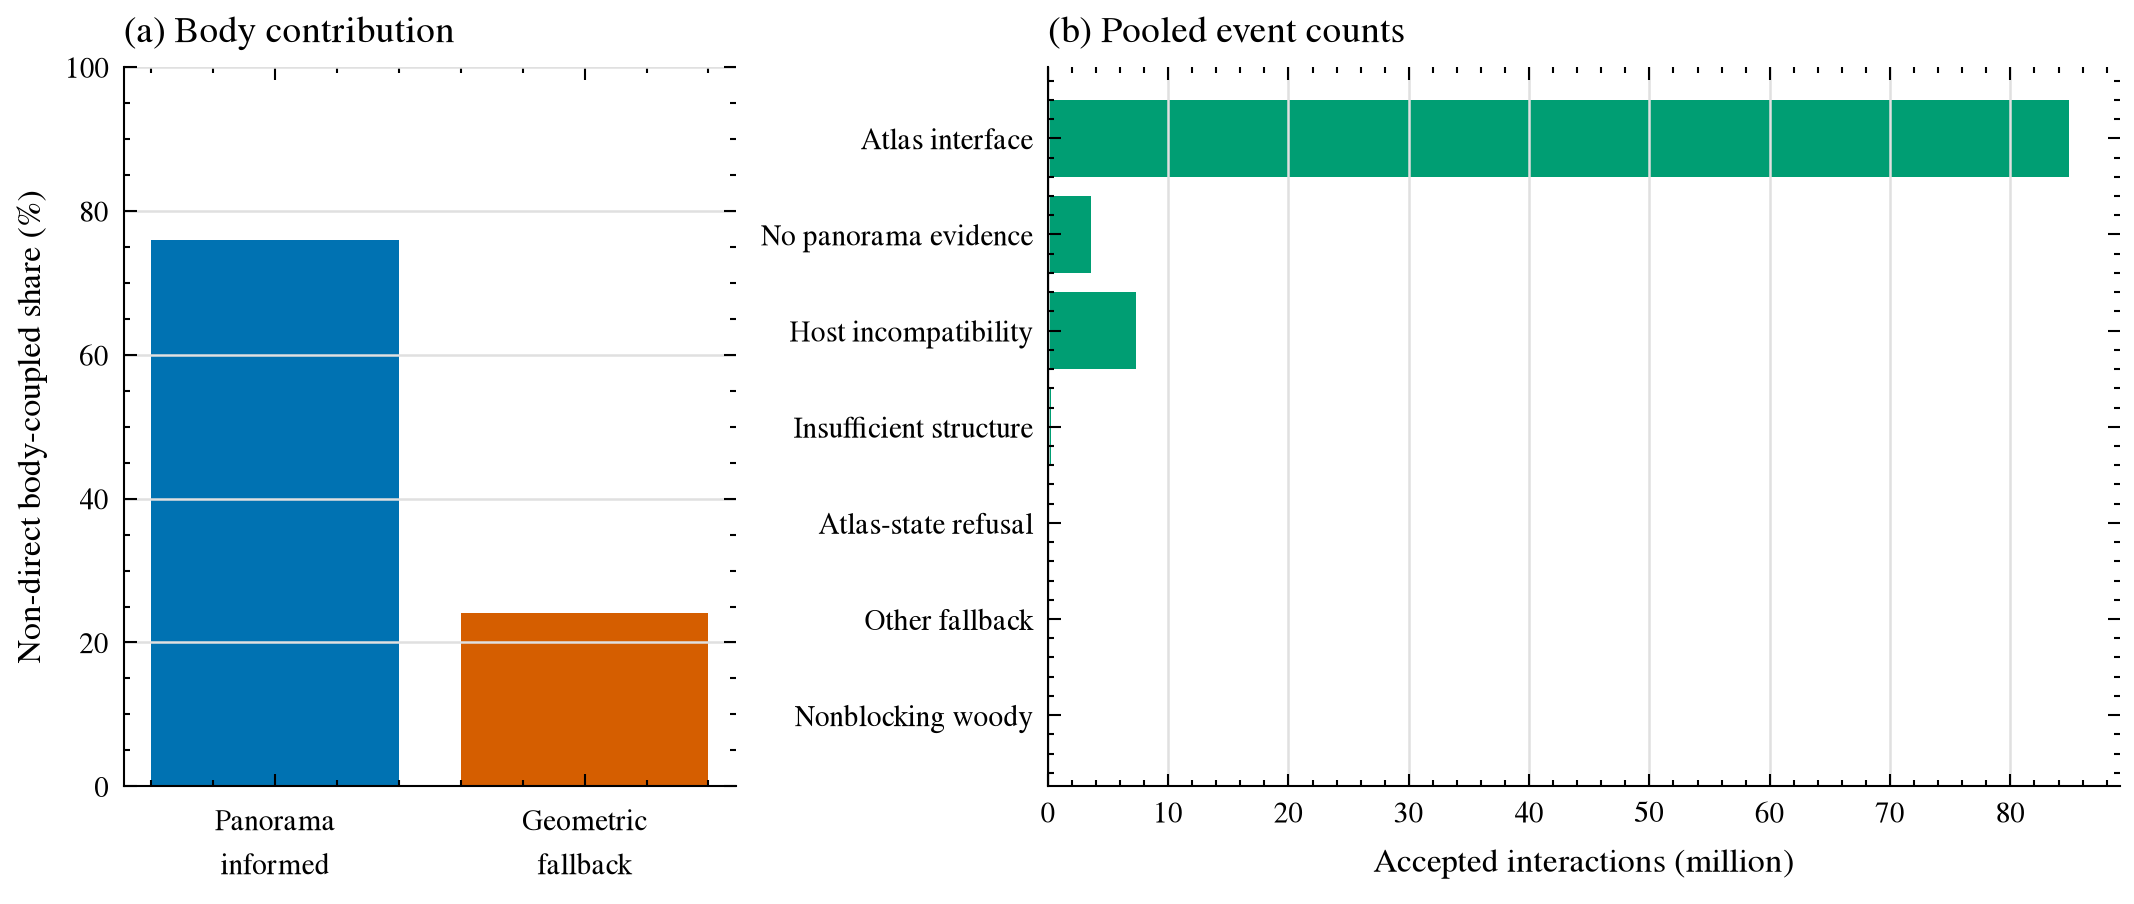
\includegraphics[width=\textwidth]{figures/ray_reached_evidence/ray_reached_evidence.pdf}
  \caption{Material labels on surfaces reached by modeled paths. Panel (a) partitions the
  pooled non-direct body-coupled whole-body SAR contribution between
  image-mapped and geometry-based materials. Panel
  (b) gives accepted retained interaction counts for all seven audit
  categories. Direct transport is not applicable because it has no material
  interaction.}
  \label{fig:si-ray-reached-coverage}
\end{figure*}

\section{Street-image alignment and acceptance}
\label{sec:si-registration}

The alignment matches the segmented sky boundary in a 360-degree street image
to the upper edge of the city mesh. The stored residual is the angular skyline
error. An accepted camera pose has a residual no greater than $4^\circ$. The second
test casts the directions labeled as sky from the fitted camera into the mesh.
It records the fraction that hits geometry and the median range of those hits.
A camera is classified as inside the geometry when the hit fraction is greater
than 0.5 and the median range is less than 2 m. The paired condition matters
because a camera inside a wall can still obtain a small silhouette residual.
A large conflict at long range is recorded as a separate low-quality state.

The current acceptance policy also requires complete sky checks and a best-fit
camera height inside the tested altitude interval. It rejects a
pose with a missing residual, a residual above $4^\circ$, missing sky
diagnostics, the near inside-geometry signature, or an optimum at the altitude
bound. Each material map stores the policy version that selected its cameras.
New builds use \texttt{registration-admission-v2}. The verified Korenmarkt map
uses its recorded version-1 policy. An accepted
camera can still be skipped if its dense and SAM label images are missing,
incomplete, malformed, or inconsistent with the fixed vocabulary. These
rejections prevent an image, pose, model, or mesh mismatch from entering the
combined material map.

\section{Numerical settings and file verification}
\label{sec:si-configuration}

\begin{table*}[!t]
  \caption{Configuration of the verified five-site result.}
  \label{tab:si-configuration}
  \centering
  \begin{tabular}{p{0.24\textwidth}p{0.70\textwidth}}
    \toprule
    Item & Production value \\
    \midrule
    Sites and routes & Korenmarkt, Prague, Madrid, Mexico City, and Tokyo Hachiko. The fixed routes contain 10, 22, 14, 11, and 16 route points. \\
    Geometry and frequency & Original photogrammetric city mesh within a 250 m horizontal radius at 15 GHz. The circular crop area is $196{,}349.54\,\mathrm{m^2}$. \\
    Transmitter model & Roofline visible from the route. Areal density sets the expected number of transmitters. Physical three-dimensional roofline length assigns their relative probability to each segment. \\
    Exposure normalization & Per unit $\rho_A P_{\mathrm{EIRP}}$. Normalized whole-body SAR has unit $\mathrm{m^2\,kg^{-1}}$. \\
    Transport & Exact direct term, exact one-reflection specular term, and stochastic next-event estimation of one diffuse reflection at the first blocking surface. \\
    Surface model & Image-derived material map with measured finish roughness. The material probabilities are evaluated at the exact hit point. \\
    Monte Carlo & 200,000 IID primary rays per route point and replica. Seeds 7 through 22 give 16 replicas. Stored convergence results use 4, 8, 12, and 16 replicas. \\
    Angular output & 4,096 passive cells collect only the first-diffuse estimate. Exact direct and one-reflection specular paths retain their arrival directions. The cells do not control launch directions. \\
    Body & Duke with 56,024 surface elements, area $1.87250\,\mathrm{m^2}$, mass 72.4 kg, and $T_0=0.500140$. The phantom faces along the walk. Body coupling uses the level-2 surface-field model. \\
    \bottomrule
  \end{tabular}
\end{table*}

The receiver is $1.5\,$m above the city surface. Route points are placed at
approximately $6\,$m intervals along the route, with aligned street-image
positions retained as route anchors. The visible-roofline calculation finds boundary
and crease edges that separate the first visible mesh hit from sky. Duplicate
mesh-edge contacts are combined. The resulting three-dimensional edge
lengths are the numerical weights. Each possible transmitter position is shifted vertically by
$0.5\,$m to avoid self-occlusion. Table~\ref{tab:si-source-quadrature} gives the
retained counts.

\begin{table}[!t]
  \caption{Number of route points and roofline segments.}
  \label{tab:si-source-quadrature}
  \centering
  \begin{tabular}{lrrr}
    \toprule
    Site & Route points & Roofline segments & Length (m) \\
    \midrule
    Korenmarkt & 10 & 457 & 157.54 \\
    Prague & 22 & 502 & 267.15 \\
    Madrid & 14 & 207 & 79.40 \\
    Mexico City & 11 & 164 & 63.69 \\
    Tokyo Hachiko & 16 & 400 & 248.76 \\
    \bottomrule
  \end{tabular}
\end{table}

The first-diffuse term uses a reciprocal next-event estimator. For each
primary direction $\mathbf u_n$ drawn uniformly over $4\pi$, the tracer keeps
the first blocking surface. It then draws one roofline segment from the
arc-length weights and tests the connecting segment. If the connection is
visible, its unscaled contribution is
\begin{equation}
  w_n = \frac{R_n(1-\kappa_n)}{\pi}
  \frac{[\mathbf n_n\!\cdot\!\mathbf d_n]_+}{r_n^2}.
\end{equation}
Here $R_n$ is the unpolarized Fresnel power reflectance, $\kappa_n$ is the
coherent specular share, $\mathbf d_n$ points from the surface to the sampled
transmitter position, and $r_n$ is the connecting distance. Occluded connections contribute
zero. The estimate is $(4\pi/N)\sum_n w_n$. The launch direction determines the
physical arrival direction by reciprocity. Only these sampled first-diffuse
contributions are accumulated in the 4,096-cell Fibonacci grid. Direct sources
and accepted one-reflection specular paths retain their exact arrival directions.

For incidence cosine $c$, complex relative permittivity $\epsilon_r$, surface
root $q=\sqrt{\epsilon_r-(1-c^2)}$, and wavelength $\lambda$, the production
law is
\begin{align}
 R &= \tfrac12\left(\left|\frac{c-q}{c+q}\right|^2+
 \left|\frac{\epsilon_r c-q}{\epsilon_r c+q}\right|^2\right), \\
 \kappa &= \exp\!\left[-\left(\frac{4\pi s c}{\lambda}\right)^2\right].
\end{align}
Thus the reflected specular and diffuse shares are $R\kappa$ and
$R(1-\kappa)$. The surface-finish roughness $s$ excludes larger periodic relief.
Table~\ref{tab:si-materials} gives the evaluated 15 GHz material table. Metal
uses the finite-conductivity value in the same complex-permittivity convention.

\begin{table*}[!t]
  \caption{Evaluated transport materials at 15 GHz. The roughness column is RMS height.}
  \label{tab:si-materials}
  \centering
  \begin{tabular}{lrrr@{\qquad}lrrr}
    \toprule
    Class & $\Re\epsilon_r$ & $-\Im\epsilon_r$ & $s$ ($\mu$m) & Class & $\Re\epsilon_r$ & $-\Im\epsilon_r$ & $s$ ($\mu$m) \\
    \midrule
    Asphalt concrete & 4.83 & 0.569 & 450 & Metal & 1.00 & $1.20\!\times\!10^7$ & 5 \\
    Brick & 3.91 & 0.044 & 30 & Plasterboard & 2.73 & 0.130 & 150 \\
    Ceramic & 7.07 & 0.081 & 280 & Plywood & 2.71 & 0.396 & 50 \\
    Chipboard & 2.58 & 0.215 & 50 & Polymer & 1.99 & 0.103 & 50 \\
    Concrete & 5.24 & 0.461 & 600 & Soil & 5.24 & 0.461 & 600 \\
    Fabric & 1.99 & 0.103 & 50 & Water & 5.24 & 0.461 & 600 \\
    Glass & 6.31 & 0.162 & 1 & Wood & 1.99 & 0.103 & 50 \\
    Marble & 7.07 & 0.081 & 280 & & & & \\
    \bottomrule
  \end{tabular}
\end{table*}

The deterministic order-1 search uses a conservative mirrored-receiver
triangle-cone broad phase when the candidate set reaches 20,000. Its CUDA
Float64 implementation leaves the host exact final test unchanged. The normal
adaptive candidate budget is 120 million. One Tokyo route point has zero
accepted order-1 paths, so a relative stopping rule cannot close around zero.
That case records and fully enumerates a 320 million candidate cap. Body
coupling uses fixed blocks of 512 directions. Candidate caps, broad-phase
thresholds, chunks, and block sizes control computation. They do not change the
stated physical model.

The result contains 73 route points, 1,168 point-replica fields, 80
site-replica runs, and 233.6 million stochastic primary rays. Every campaign
manifest lists 42 files. All 210 recorded file hashes pass. The aggregate JSON,
CSV, PDF, and PNG also match their artifact manifest. Across the 1,168 fields,
the maximum raw residual between the saved total and the sum of direct,
all-specular, and first-diffuse components is
$1.735\times10^{-18}\,\mathrm{m^{-2}}$. The CUDA body result agrees with the
NumPy reference to a maximum relative error of $6.64\times10^{-16}$ in the
verified benchmark. The verified artifacts are stored under
the roofline campaign output package named
\texttt{current\_five\_city\_\allowbreak{}first\_material\_interaction}.
The Duke STL has SHA-256
\texttt{781e65ef3882f134\allowbreak{}7669e0ddca5dafa82\allowbreak{}cd6368dddd6b9e80\allowbreak{}1dc49613822fe3b}.
The verified body-area array has SHA-256
\texttt{5dd410b9512fdb02\allowbreak{}74dd1ac1fb8f7b70\allowbreak{}87564abfed998d57\allowbreak{}a25065e87ffebd6a}.
Each calculation manifest also verifies the city mesh, material map, roofline
segments, source weights, route arrays, material tables, and executable configuration.

\section{Replica convergence and lower tails}
\label{sec:si-convergence}

% claim: replica_convergence_48_to_64
\begin{table}[!t]
  \caption{Convergence from 48 to 64 replicas. Bootstrap width is the 95\% interval width for route $q_{10}$ whole-body SAR. Shadow change is the largest stepwise change among the six shadowed route points.}
  \label{tab:si-convergence}
  \centering
  \begin{tabular}{lrrr}
    \toprule
    Site & \shortstack{$q_{10}$ change\\(dB)} & \shortstack{Bootstrap width\\(dB)} & \shortstack{Shadow change\\(dB)} \\
    \midrule
    Korenmarkt & 0.0000723 & 0.000222 & -- \\
    Prague & 0.0000203 & 0.000218 & -- \\
    Madrid & 0.00000615 & 0.000378 & -- \\
    Mexico City & 0.00344 & 0.364 & 0.0125 \\
    Tokyo Hachiko & 0.00491 & 0.0538 & 0.0104 \\
    \bottomrule
  \end{tabular}
\end{table}

The 64-replica extension uses seeds 7 through 70 and nested looks of 16, 24,
32, 48, and 64. Its first 16 replicas exactly match the verified campaign
arrays after timing fields are removed. Mexico City route points 0, 1, and 3
and Tokyo Hachiko route points 13, 14, and 15 remain the six shadowed points.
The first-diffuse estimate is their only nonzero modeled contribution.
From 48 to 64 replicas, their largest pointwise whole-body SAR changes are
0.0125 and 0.0104~dB. The route $q_{10}$ changes are 0.00344 and 0.00491~dB,
and their whole-replica bootstrap widths are 0.364 and 0.0538~dB.

The bootstrap resamples complete replicas jointly over all route points, so it
preserves spatial dependence within one replica. Its 2,000 draws use PCG64 with
the authenticated analysis seed 20260814. All five identities, manifests,
component closures, and common inputs pass, and both lower tails meet the
stated 48-to-64 aggregate criteria. Mexico City nevertheless retains
rare-event first-diffuse behavior: its maximum positive replica contribution
is 5738 times its positive-replica median, compared with 2.38 for Tokyo
Hachiko. These intervals apply to each fixed route.
They do not include route-selection or city-sampling uncertainty.

\begin{figure*}[!t]
  \centering
  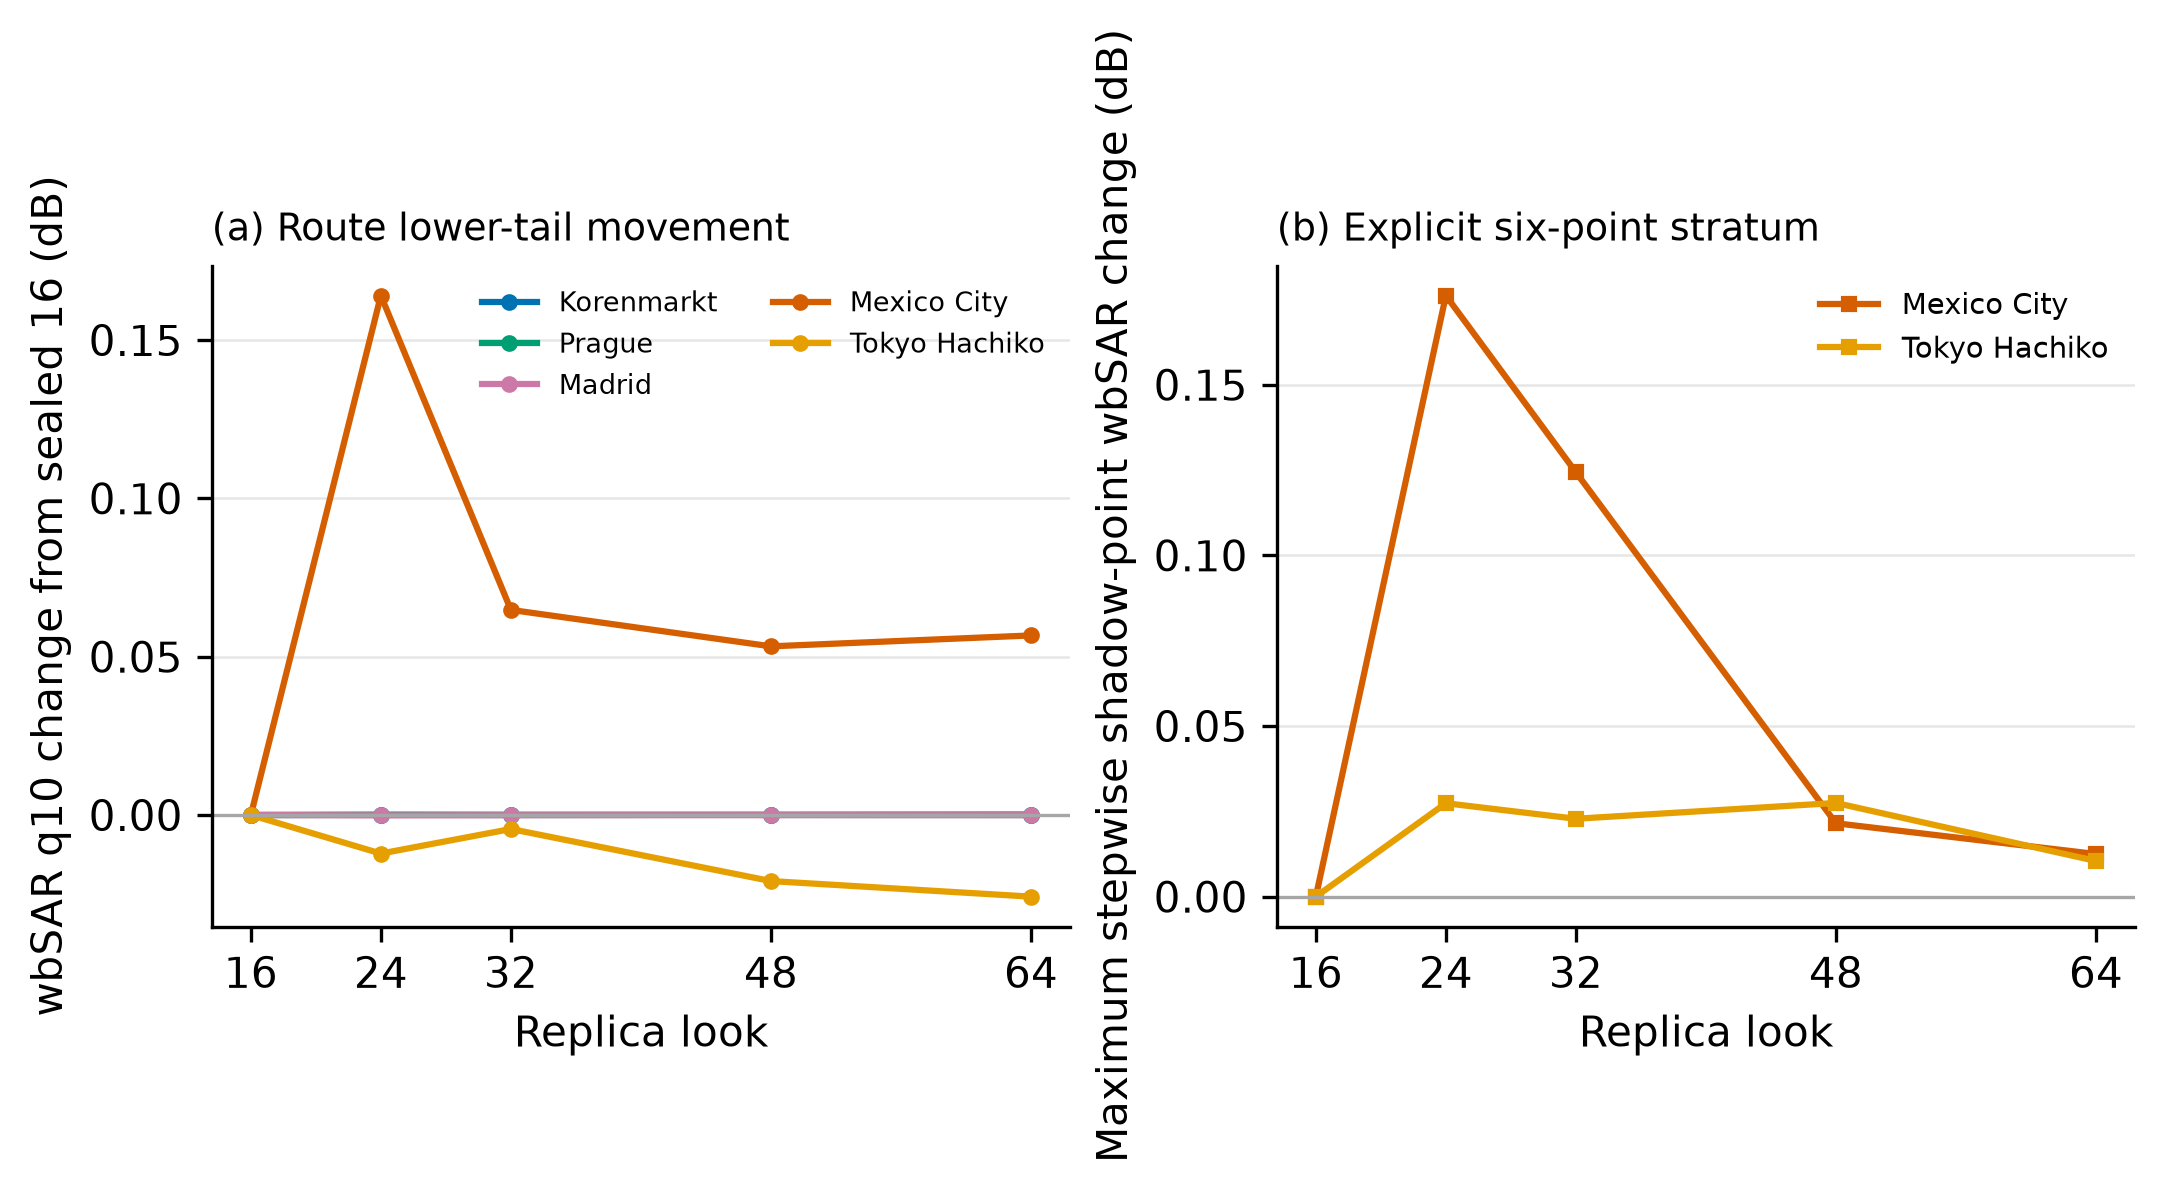
\includegraphics[width=\textwidth]{figures/convergence64/convergence64.pdf}
  \caption{Convergence through 64 replicas. Panel (a) shows
  route $q_{10}$ whole-body SAR changes from the verified 16-replica value. Panel
  (b) shows the largest stepwise change among the three shadowed route points in
  each of Mexico City and Tokyo Hachiko. The final 48-to-64 changes satisfy the
  stated aggregate lower-tail criteria. Mexico City retains rare-event
  first-diffuse behavior.}
  \label{fig:si-convergence}
\end{figure*}

\section{Primary-ray and angular-cell budgets}
\label{sec:si-budget-sensitivity}

% claim: roofline_budget_sensitivity
The budget test used paired seeds and common random numbers at the Madrid,
Mexico City, and Prague routes. Exact direct and all-specular components were
byte identical in every paired comparison, and the 200,000-ray, 4,096-cell
replay matched the verified baseline. The largest route-median whole-body-SAR
change among the five cheaper settings was 0.000797345~dB. The directional
first-diffuse fields did not pass the stated test. The largest site $q_{90}$
normalized-$L_{1}$ differences were 0.877498, 0.678942, and 0.400218 at 25,000,
50,000, and 100,000 rays, respectively. At 1,024 and 2,048 cells, they were
0.491265 and 0.455431. Each value exceeds the 0.1 limit. The largest absolute
whole-body-SAR changes at a shadowed Mexico City point were 0.707362, 0.563841,
and 0.217259~dB for the three ray settings. They were 0.00206975 and
0.00088674~dB for the two cell settings.

Ray cuts also do not give a defensible end-to-end speedup. At 25,000 rays, estimator-wall-time ratios relative to the baseline range from 0.991 to 1.064 across the three routes. Exact all-specular work takes 8.06 to 23.79~s in the baseline, whereas stochastic tracing takes 1.15 to 2.40~s. The $q_{90}$ variance-time ratios for every ray-reduced arm exceed one, with a minimum of 3.16. The reported timing therefore leaves the exact specular stage dominant while the reduced ray settings increase first-diffuse variance. Figure~\ref{fig:si-budget-sensitivity} retains the 200,000-ray, 4,096-cell setting as the production baseline.

\begin{figure*}[!t]
  \centering
  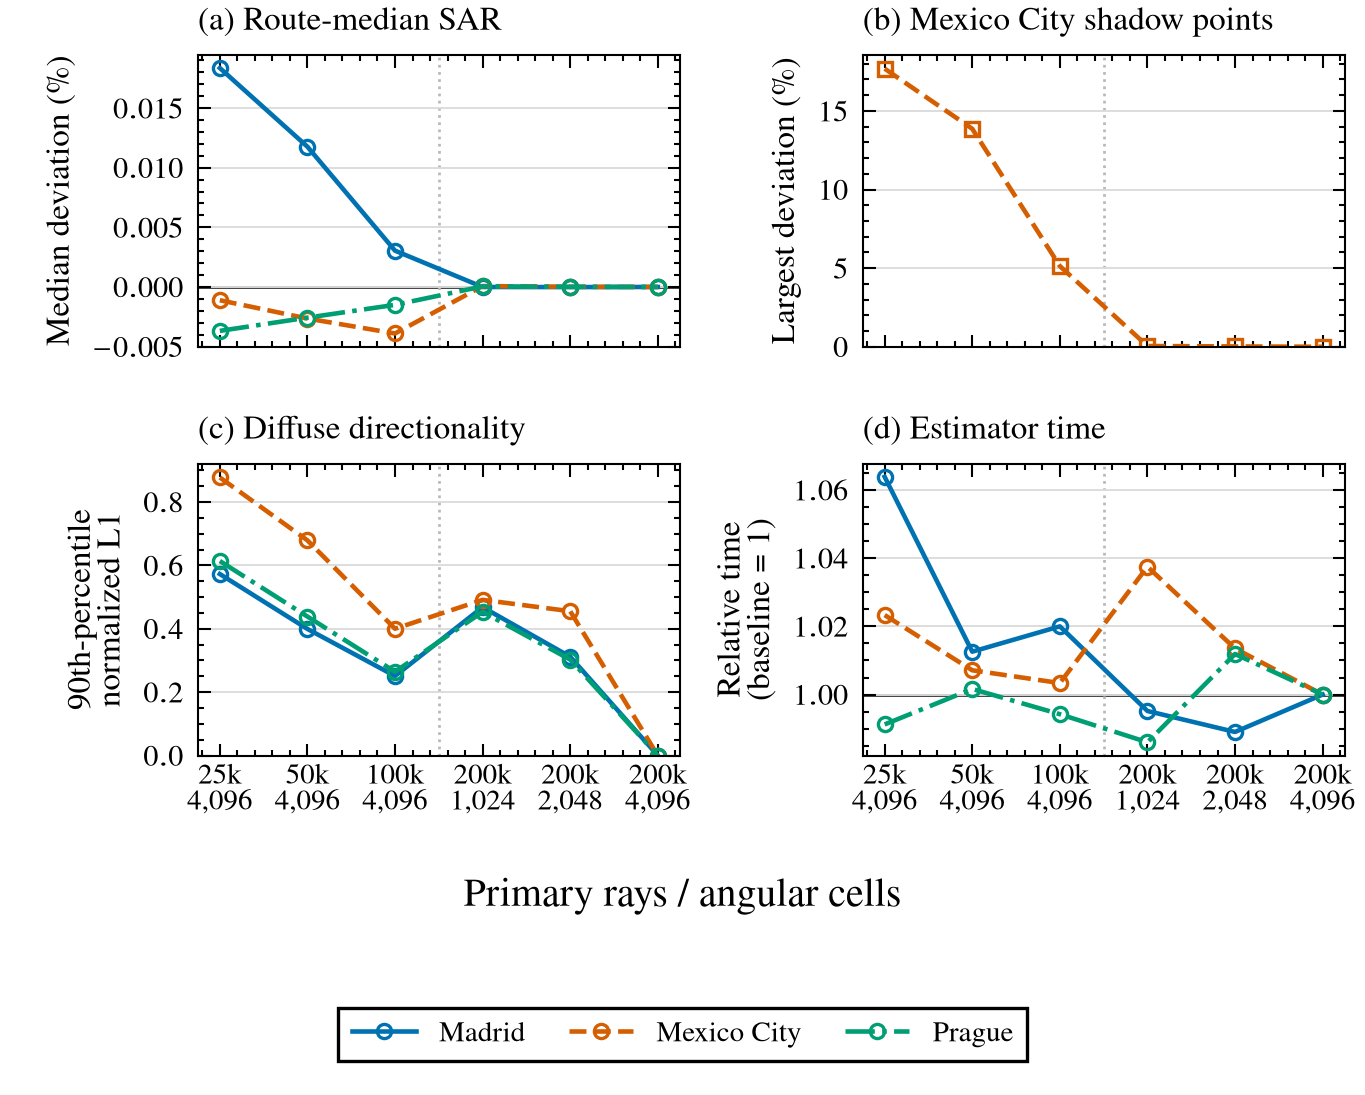
\includegraphics[width=\textwidth]{figures/budget_sensitivity/budget_sensitivity.pdf}
  \caption{Primary-ray and angular-cell budget sensitivity under the current first-material transport contract. All five cheaper settings leave route-median whole-body SAR nearly unchanged, but each exceeds the directional first-diffuse gate. Exact direct and order-1 specular components remain invariant. The diagnostic retains 200,000 rays and 4,096 cells.}
  \label{fig:si-budget-sensitivity}
\end{figure*}

\section{Paired material-map control}
\label{sec:si-material-control}

The control replaces the image-derived material map with geometry-based
materials in Madrid and Mexico City. Each pair keeps the city mesh, route,
source curve, source weights, body, frequency, transport steps, ray count,
output cells, and 16 seeds fixed. A strict compatibility check permits changes
only in the material mode, the material arrays and hashes, the run
configuration, and the presence of the material-map files. Both paired manifests pass
all 42 file hashes. The comparison therefore measures sensitivity to the
image-derived material map under the current model. It does not isolate reflectance because
the map also changes roughness, specular share, and the nonblocking state of
woody vegetation. It does not measure semantic or material accuracy.

\begin{table}[!t]
  \caption{Image-to-geometry change in route quantiles of normalized
  whole-body SAR. Positive values mean that the image-derived result is larger.}
  \label{tab:si-material-control}
  \centering
  \begin{tabular}{lrrr}
    \toprule
    Site & q10 (dB) & q50 (dB) & q90 (dB) \\
    \midrule
    Madrid & 0.233 & 0.249 & 0.269 \\
    Mexico City & 24.84 & -0.158 & 0.104 \\
    \bottomrule
  \end{tabular}
\end{table}

The direct component is identical within each pair. In Madrid, the image-derived map raises
the route-median all-specular whole-body SAR by 1.89 dB and lowers the
first-diffuse component by 12.43 dB. Their combined effect changes the total
route median by 0.249 dB. Mexico City's 24.84 dB q10 change is set by three
shadowed route points where both alternatives are near zero and first-diffuse
transport is the only nonzero modeled contribution. The Mexico City median and q90
changes are $-0.158$ and 0.104 dB. The two sites show that component changes can
be much larger than the change in total normalized whole-body SAR. The result
supports a material-map sensitivity statement for these routes only.

\FloatBarrier
\section{Separate geometric fixed-grid diagnostic}
\label{sec:si-geometric-screening}

% claim: geometric_fixed_grid_diagnostic
A separate diagnostic describes ten urban locations with a deterministic point
design. At each location, the calculation builds a complete 6~m walkable-ground
lattice within 90~m and retains 64 observation points evenly across its
nearest-neighbor ordering. The visible roofline transmitter curve is built from
these same 64 points. Surface properties use geometry-based priors, and the
Duke phantom faces north at every point. The calculation uses the same
first-material transport model with 16 seeds, 200,000 primary rays per point
and seed, and 4,096 first-diffuse output cells. The fixed-grid design remains
separate from the pedestrian-route calculations and is not combined with the
five-route results.

Across the ten fixed-grid descriptions, the ratio of the largest to smallest
normalized whole-body-SAR quantile is 2.02 for $q_{10}$, 2.01 for $q_{50}$,
and 2.23 for $q_{90}$. The pooled component shares range from 75.2\% to
80.6\% for direct transport, 13.1\% to 19.6\% for order-1 specular transport,
and 4.1\% to 7.1\% for first-diffuse transport.

Changing the design from 16 to 64 points, evaluated with the first four seeds,
moved the site quantiles by at most 2.26~dB for $q_{10}$, 1.38~dB for
$q_{50}$, and 3.47~dB for $q_{90}$. By contrast, the change from eight to
16 seeds moved them by at most 0.0036, 0.0017, and 0.0020~dB. With the
64-point transmitter curve fixed, the change from 32 to 64 receiver points was
as large as 1.36, 0.219, and 0.636~dB. The calculation is therefore far more
sensitive to point selection than to the number of seeds.

Each quantile describes exactly 64 fixed observation points. Its reported
conditional Monte Carlo standard error is the sample standard deviation of the
16 within-seed 64-point quantiles divided by $\sqrt{16}$. This standard error
is not total uncertainty. It does not include uncertainty from the grid design,
body orientation, material
priors, or transmitter-curve design. The values therefore describe only the
declared fixed-grid calculation.

\begin{figure*}[!t]
  \centering
  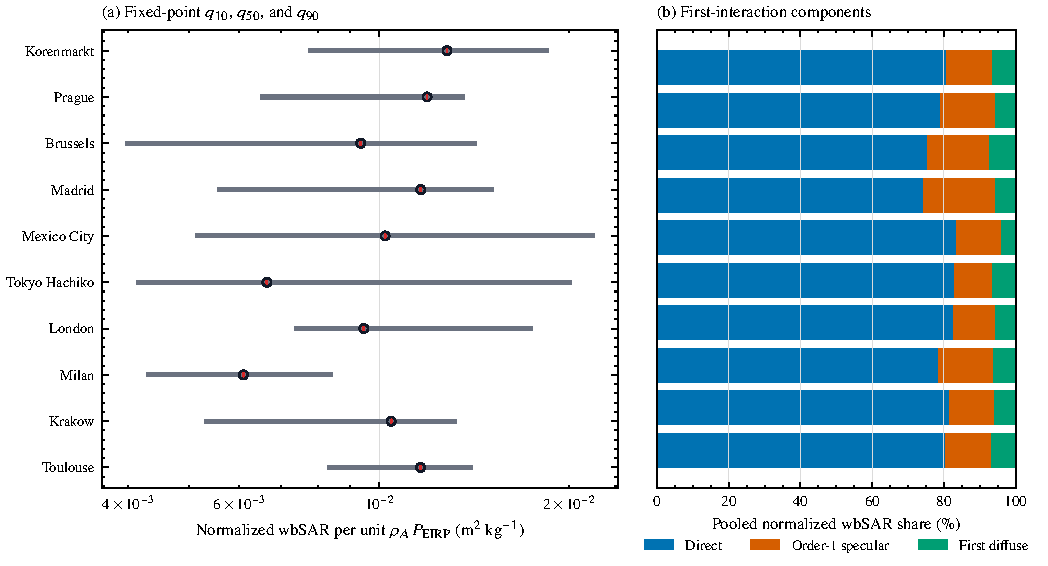
\includegraphics[width=\textwidth]{figures/geometric_screening/geometric_screening.pdf}
  \caption{Separate geometric fixed-grid diagnostic at ten urban locations.
  Panel (a) shows $q_{10}$, $q_{50}$, and $q_{90}$ across the 64 fixed
  observation points. Red bars give the 16-seed conditional Monte Carlo
  standard error of $q_{50}$. Panel (b) shows the pooled additive component
  shares. These results are not combined with the five-route calculation.}
  \label{fig:si-geometric-screening}
\end{figure*}

\section{Computation time}
\label{sec:si-timing}

The repeated numerical campaigns start from a ready city scene. Their wall
times on one A6000 are 29.79 s for Korenmarkt, 69.02 s for Prague, 40.70 s for
Madrid, 30.92 s for Mexico City, and 50.11 s for Tokyo Hachiko. These times
include the 16 transport replicas and body coupling for the complete fixed
route. They exclude image and mesh acquisition, image-to-mesh alignment,
image labeling, depth processing, and material-map construction. Persistent
transport caches and exact conservative broad-phase screening reduce repeated
work with no change to the saved scientific arrays.

The full scene-preparation path has no complete timing record. Available 14-image
records give 21.3 to 26.6 min for the hybrid semantic pass and 5.3 to 13.6 min
for material-map construction. Acquisition, alignment, depth, and combination were not
all timed separately. One live A6000 parity check took 116.981 s for one
image with independent model sessions. A shared session processed two
images in 199.228 s and reproduced every scientific image array, concept
cache array, prompt gate, and normalized metadata field exactly. These values
are implementation checks. They do not define a universal time per image.
A single cold end-to-end time is therefore not reported.

\balance
\section{Additional limitations}
\label{sec:si-limitations}

The transport result contains exact direct transport, exact one-reflection
specular transport, and one diffuse reflection. A sampled first-diffuse path
stops at that reflection. The model omits a specular reflection after the
diffuse event, further specular reflections, and all other multipath. The controlled open-square
test validates the first-diffuse normalization, visibility, inverse-square loss,
and cosine factors. The maximum adjoint-versus-Sionna difference is 0.0621 dB
for the bounced term and 0.0344 dB for total transport in that test. The same
three-way test has not been repeated for the full five-site calculation with its
image-derived materials and exact specular term. The test validates this component. It
does not provide external validation of every city result. The level-2 body
coupling uses one-sided local incidence. It does not trace body self-occlusion.

The five routes are selected case studies. Their differences do not rank the
five cities and do not estimate population exposure. Each result is normalized
per unit $\rho_A P_{\mathrm{EIRP}}$, so it is not an absolute prediction for an
operator deployment. The study uses one 15 GHz frequency, one body phantom,
one body orientation that faces along the walk, one roofline transmitter model, and five
plaza routes. Additional frequencies, body models, headings, deployment laws,
street canyons, parks, and repeated route selections are outside this study.

Image-derived materials cover only surfaces that an accepted camera can see and
project onto the city mesh. Unlabeled material-map cells use the geometry-based
material. Transient pixels do not enter the static surface. Image labels can
preserve within-triangle material variation, but it cannot recover geometry
that is absent from the photogrammetric mesh. The two-site material control
tests how these assignments change the final result, but it supplies no image-label
ground truth. Coverage over the complete city mesh also differs from coverage
on the surfaces reached by propagation paths. The path audit reports where the
recorded image-derived and geometry-based materials act in one-reflection
specular and first-diffuse transport. It does not test whether the image labels
or geometry-based material are correct. The current claims therefore apply to
these recorded surfaces.

\clearpage

% End of supplementary-information body.
